\documentclass[14pt]{extbook}
\usepackage{multicol, enumerate, enumitem, hyperref, color, soul, setspace, parskip, fancyhdr} %General Packages
\usepackage{amssymb, amsthm, amsmath, bbm, latexsym, units, mathtools} %Math Packages
\everymath{\displaystyle} %All math in Display Style
% Packages with additional options
\usepackage[headsep=0.5cm,headheight=12pt, left=1 in,right= 1 in,top= 1 in,bottom= 1 in]{geometry}
\usepackage[usenames,dvipsnames]{xcolor}
\usepackage{dashrule}  % Package to use the command below to create lines between items
\newcommand{\litem}[1]{\item#1\hspace*{-1cm}\rule{\textwidth}{0.4pt}}
\pagestyle{fancy}
\lhead{Makeup Progress Quiz -1}
\chead{}
\rhead{Version C}
\lfoot{7547-2949}
\cfoot{}
\rfoot{Fall 2020}
\begin{document}

\begin{enumerate}
\litem{
Determine the horizontal and/or oblique asymptotes in the rational function below.\[ f(x) = \frac{8x^{3} -30 x^{2} +13 x + 30}{4x^{2} -5 x -6} \]\begin{enumerate}[label=\Alph*.]
\item \( \text{Horizontal Asymptote of } y = 2.0 \text{ and Oblique Asymptote of } y = 2x -5 \)
\item \( \text{Horizontal Asymptote of } y = 2.0 \text{ and Oblique Asymptote of } y = 2x -5 \)
\item \( \text{Horizontal Asymptote of } y = 2.0  \)
\item \( \text{Oblique Asymptote of } y = 2x -5. \)
\item \( \text{Horizontal Asymptote at } y = 2.0 \)

\end{enumerate} }
\litem{
Determine the horizontal and/or oblique asymptotes in the rational function below.\[ f(x) = \frac{8x^{3} -46 x^{2} +41 x + 60}{4x^{3} +22 x^{2} -64 x -48} \]\begin{enumerate}[label=\Alph*.]
\item \( \text{Horizontal Asymptote of } y = 0  \)
\item \( \text{Vertical Asymptote of } y = -4.000  \)
\item \( \text{None of the above} \)
\item \( \text{Horizontal Asymptote of } y = 2.000  \)
\item \( \text{Vertical Asymptote of } y = 4  \)

\end{enumerate} }
\litem{
Which of the following functions \textit{could} be the graph below?
\begin{center}
    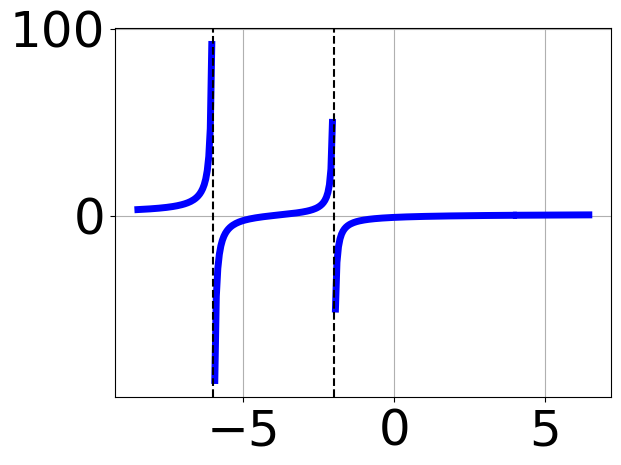
\includegraphics[width=0.5\textwidth]{../Figures/identifyGraphOfRationalFunctionC.png}
\end{center}
\begin{enumerate}[label=\Alph*.]
\item \( f(x)=\frac{x^{3} +6 x^{2} -7 x -60}{x^{3} +4 x^{2} -20 x -48} \)
\item \( f(x)=\frac{x^{3} -3 x^{2} -16 x + 48}{x^{3} +4 x^{2} -20 x -48} \)
\item \( f(x)=\frac{x^{3} +3 x^{2} -16 x -48}{x^{3} -4 x^{2} -20 x + 48} \)
\item \( f(x)=\frac{x^{3} +3 x^{2} -16 x -48}{x^{3} -4 x^{2} -20 x + 48} \)
\item \( \text{None of the above are possible equations for the graph.} \)

\end{enumerate} }
\litem{
Determine the horizontal and/or oblique asymptotes in the rational function below.\[ f(x) = \frac{12x^{3} -41 x^{2} +44 x -15}{3x^{2} -11 x + 10} \]\begin{enumerate}[label=\Alph*.]
\item \( \text{Horizontal Asymptote of } y = 4.0  \)
\item \( \text{Horizontal Asymptote at } y = 2.0 \)
\item \( \text{Horizontal Asymptote of } y = 4.0 \text{ and Oblique Asymptote of } y = 4x + 1 \)
\item \( \text{Oblique Asymptote of } y = 4x + 1. \)
\item \( \text{Horizontal Asymptote of } y = 2.0 \text{ and Oblique Asymptote of } y = 4x + 1 \)

\end{enumerate} }
\litem{
Determine the vertical asymptotes and holes in the rational function below.\[ f(x) = \frac{6x^{3} +31 x^{2} +8 x -80}{9x^{2} -16} \]\begin{enumerate}[label=\Alph*.]
\item \( \text{Vertical Asymptote of } x = -1.333 \text{ and hole at } x = 1.333 \)
\item \( \text{Vertical Asymptote of } x = 0.667 \text{ and hole at } x = 1.333 \)
\item \( \text{Holes at } x = -1.333 \text{ and } x = 1.333 \text{ with no vertical asymptotes.} \)
\item \( \text{Vertical Asymptotes of } x = -1.333 \text{ and } x = 1.333 \text{ with no holes.} \)
\item \( \text{Vertical Asymptotes of } x = -1.333 \text{ and } x = -2.5 \text{ with a hole at } x = 1.333 \)

\end{enumerate} }
\litem{
Determine the vertical asymptotes and holes in the rational function below.\[ f(x) = \frac{4x^{3} -28 x^{2} +63 x -45}{6x^{2} -11 x -10} \]\begin{enumerate}[label=\Alph*.]
\item \( \text{Vertical Asymptotes of } x = -0.667 \text{ and } x = 2.5 \text{ with no holes.} \)
\item \( \text{Vertical Asymptote of } x = -0.667 \text{ and hole at } x = 2.5 \)
\item \( \text{Holes at } x = -0.667 \text{ and } x = 2.5 \text{ with no vertical asymptotes.} \)
\item \( \text{Vertical Asymptotes of } x = -0.667 \text{ and } x = 1.5 \text{ with a hole at } x = 2.5 \)
\item \( \text{Vertical Asymptote of } x = 0.667 \text{ and hole at } x = 2.5 \)

\end{enumerate} }
\litem{
Determine the horizontal and/or oblique asymptotes in the rational function below.\[ f(x) = \frac{2x^{2} +7 x -15}{12x^{3} +20 x^{2} -97 x + 60} \]\begin{enumerate}[label=\Alph*.]
\item \( \text{Oblique Asymptote of } y = 6x -11. \)
\item \( \text{Horizontal Asymptote of } y = 0.167 \text{ and Oblique Asymptote of } y = 6x -11 \)
\item \( \text{Horizontal Asymptote of } y = 0.167  \)
\item \( \text{Horizontal Asymptote at } y = -5.000 \)
\item \( \text{Horizontal Asymptote of } y = 0 \)

\end{enumerate} }
\litem{
Which of the following functions \textit{could} be the graph below?
\begin{center}
    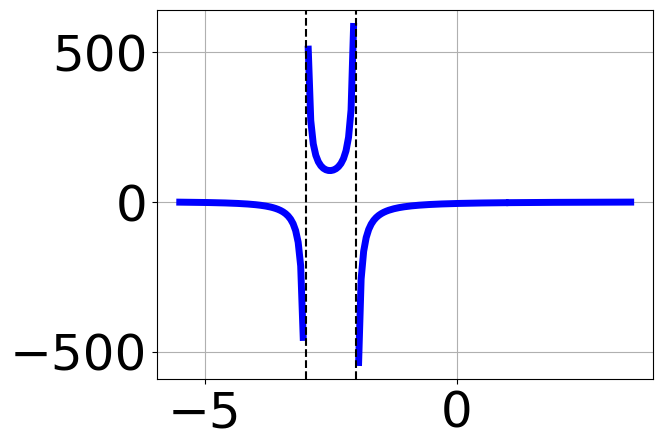
\includegraphics[width=0.5\textwidth]{../Figures/identifyGraphOfRationalFunctionCopyC.png}
\end{center}
\begin{enumerate}[label=\Alph*.]
\item \( f(x)=\frac{x^{3} -31 x + 30}{x^{3} +4 x^{2} +x -6} \)
\item \( f(x)=\frac{x^{3} -31 x -30}{x^{3} -4 x^{2} +x + 6} \)
\item \( f(x)=\frac{x^{3} -4 x^{2} -35 x + 150}{x^{3} +4 x^{2} +x -6} \)
\item \( f(x)=\frac{x^{3} -31 x -30}{x^{3} -4 x^{2} +x + 6} \)
\item \( \text{None of the above are possible equations for the graph.} \)

\end{enumerate} }
\litem{
Determine the vertical asymptotes and holes in the rational function below.\[ f(x) = \frac{9x^{3} -15 x^{2} -2 x + 8}{9x^{2} -9 x -10} \]\begin{enumerate}[label=\Alph*.]
\item \( \text{Holes at } x = 1.667 \text{ and } x = -0.667 \text{ with no vertical asymptotes.} \)
\item \( \text{Vertical Asymptote of } x = 1.0 \text{ and hole at } x = -0.667 \)
\item \( \text{Vertical Asymptotes of } x = 1.667 \text{ and } x = -0.667 \text{ with no holes.} \)
\item \( \text{Vertical Asymptote of } x = 1.667 \text{ and hole at } x = -0.667 \)
\item \( \text{Vertical Asymptotes of } x = 1.667 \text{ and } x = 1.333 \text{ with a hole at } x = -0.667 \)

\end{enumerate} }
\litem{
Determine the vertical asymptotes and holes in the rational function below.\[ f(x) = \frac{8x^{3} +34 x^{2} +45 x + 18}{4x^{2} -9} \]\begin{enumerate}[label=\Alph*.]
\item \( \text{Vertical Asymptote of } x = 2.0 \text{ and hole at } x = -1.5 \)
\item \( \text{Vertical Asymptote of } x = 1.5 \text{ and hole at } x = -1.5 \)
\item \( \text{Vertical Asymptotes of } x = 1.5 \text{ and } x = -1.5 \text{ with no holes.} \)
\item \( \text{Vertical Asymptotes of } x = 1.5 \text{ and } x = -0.75 \text{ with a hole at } x = -1.5 \)
\item \( \text{Holes at } x = 1.5 \text{ and } x = -1.5 \text{ with no vertical asymptotes.} \)

\end{enumerate} }
\end{enumerate}

\end{document}